% Compile with XeLaTeX. Define \WithAppendix to include four backup slides.
% Source of truth: CURRENT_BEST_MODEL.json and report v17, checked 2026-11-08.
\documentclass[aspectratio=169,20pt]{beamer}
\geometry{paperwidth=320mm,paperheight=180mm}
\usepackage{fontspec}
\setsansfont{texgyreheros}[Extension=.otf,UprightFont=*-regular,BoldFont=*-bold,ItalicFont=*-italic,BoldItalicFont=*-bolditalic]
\setmainfont{texgyreheros}[Extension=.otf,UprightFont=*-regular,BoldFont=*-bold,ItalicFont=*-italic,BoldItalicFont=*-bolditalic]
\usefonttheme{professionalfonts}
\usepackage{amsmath,amssymb,booktabs,array,graphicx}
\usepackage{unicode-math}
\setmathfont{latinmodern-math.otf}
\usepackage{tikz}
\usetikzlibrary{arrows.meta}
\definecolor{Navy}{HTML}{142D40}
\definecolor{Blue}{HTML}{0072B2}
\definecolor{Teal}{HTML}{007C78}
\definecolor{Muted}{HTML}{536675}
\definecolor{Light}{HTML}{E7EDF1}
\definecolor{Orange}{HTML}{AA4D00}
\setbeamercolor{normal text}{fg=Navy,bg=white}
\setbeamercolor{structure}{fg=Blue}
\setbeamercolor{frametitle}{fg=Navy,bg=white}
\setbeamercolor{itemize item}{fg=Blue}
\setbeamercolor{footline}{fg=Muted,bg=white}
\setbeamertemplate{navigation symbols}{}
\setbeamersize{text margin left=18mm,text margin right=18mm}
\setbeamerfont{frametitle}{size=\fontsize{29}{34},series=\bfseries}
\setbeamertemplate{frametitle}{\vspace{6mm}\insertframetitle\par\vspace{1mm}}
\setbeamertemplate{footline}{\hspace{18mm}\fontsize{11}{13}\selectfont SSU Data Dash 2026\hfill\ifnum\value{framenumber}>7 Backup \number\numexpr\value{framenumber}-7\relax\else\insertframenumber\,/\,7\fi\hspace{18mm}\vspace{5mm}}
\setbeamerfont{normal text}{size=\fontsize{20}{25}}
\setlength{\parskip}{3mm}
\newcommand{\smalltext}{\fontsize{15}{19}\selectfont}
\newcommand{\tinytext}{\fontsize{12}{15}\selectfont}
\newcommand{\eyebrow}[1]{{\fontsize{14}{17}\selectfont\color{Muted}\MakeUppercase{#1}}}
\newcommand{\takeaway}[1]{{\color{Teal}\bfseries #1}}
\newcommand{\sourceline}[1]{\par{\tinytext\color{Muted}#1\par}}
\hypersetup{pdftitle={Toronto Home-Price Prediction | SSU Data Dash 2026},pdfsubject={Final selected models; five-minute presentation},pdfauthor={},colorlinks=true,urlcolor=Blue}

\begin{document}

% 1 -- Opening and the user decisions. Target: 25 seconds.
\begin{frame}[t]
\vspace{5mm}
\eyebrow{SSU Data Dash 2026}\par
\vspace{6mm}

{\fontsize{43}{49}\selectfont\bfseries Toronto Home-Price\\Prediction\par}\par
\vspace{11mm}
\begin{columns}[T,onlytextwidth]
\begin{column}{0.47\textwidth}
{\fontsize{27}{32}\selectfont\color{Blue}\bfseries Off-market\par}\par
\vspace{3mm}
What is this home worth\\before listing?

\smalltext No asking price
\end{column}
\begin{column}{0.47\textwidth}
{\fontsize{27}{32}\selectfont\color{Teal}\bfseries List-aware\par}\par
\vspace{3mm}
What will this listing\\close at?

\smalltext Asking price available
\end{column}
\end{columns}
\vfill
{\smalltext\color{Muted}150,000 synthetic Toronto sales\quad\textbullet\quad Jan 2021--May 2026\quad\textbullet\quad No outside prediction data}
\end{frame}

% 2 -- Both validation protocols. Target: 55 seconds.
\begin{frame}[t]{Official monthly and team fixed-four-month validation}
\relax
\vspace{3mm}
{\fontsize{17}{22}\selectfont
\renewcommand{\arraystretch}{1.65}
\begin{tabular*}{\textwidth}{@{}>{\raggedright\arraybackslash}p{6cm}p{7.8cm}p{7.7cm}@{\extracolsep{\fill}}r@{}}
\toprule
\textbf{Purpose} & \textbf{Training cutoff} & \textbf{Evaluation / forecast} & \textbf{Homes}\\
\midrule
\textcolor{Blue}{Official monthly} & Before each month & Dec 2025--May 2026 & 10,069\\
\textcolor{Teal}{Team fixed four-month} & Before Feb 1, 2026 & Feb--May 2026; no updates & 7,773\\
Final refit & Before Jun 1, 2026 & Jun--Sep 2026; hidden labels & 3,974 / 4,064\\
\bottomrule
\end{tabular*}}
\vspace{6mm}
\begin{columns}[T,onlytextwidth]
\begin{column}{0.31\textwidth}
\eyebrow{Feature lookback}

\textbf{90 / 180 / 365 days}

\smalltext Past-market summaries
\end{column}
\begin{column}{0.31\textwidth}
\eyebrow{Training sample}

\textbf{Several years}

\smalltext Expanding eligible past sales
\end{column}
\begin{column}{0.31\textwidth}
\eyebrow{Forecast horizon}

\textbf{One or four months}

\smalltext Monthly refits or one frozen batch
\end{column}
\end{columns}
\vfill
{\fontsize{18}{23}\selectfont\bfseries No current-fold outcomes enter fitting or history pools.}

\sourceline{Historical queries end before min(listing date, cutoff). Settings stay fixed. Configuration selection overlapped Dec 2025, so these remain cumulative development results.}
\end{frame}

% 3 -- LightGBM overview. Target: 40 seconds.
\begin{frame}[t]{LightGBM: efficient gradient-boosted trees}
\relax
{\smalltext\color{Muted}A sequence of decision trees for tabular data.}\par
\vspace{7mm}
\begin{columns}[T,onlytextwidth]
\begin{column}{0.54\textwidth}
{\color{Blue}\bfseries 1}\quad Boosting: learn corrections

{\smalltext Each new tree learns a loss-based correction to the score.\par}
\vspace{6mm}
{\color{Blue}\bfseries 2}\quad Leaf-wise: split where it helps most

{\smalltext Grow the leaf with the largest expected loss reduction.\par}
\vspace{6mm}
{\color{Blue}\bfseries 3}\quad Histograms: search splits efficiently

{\smalltext Group numeric values into bins to reduce search cost.\par}
\end{column}
\begin{column}{0.40\textwidth}
{\color{Teal}\bfseries Why it fits our task}\par
\vspace{4mm}
Nonlinear relationships

{\smalltext Location, size and type can interact.\par}
\vspace{4mm}
Numeric and categorical inputs

{\smalltext Property attributes and local market context.\par}
\vspace{4mm}
Controlled tree complexity

{\smalltext Leaf limits, minimum samples and penalties.\par}
\end{column}
\end{columns}
\vfill
\[
\underbrace{f_m(X)}_{\text{updated score}}
=\underbrace{f_{m-1}(X)}_{\text{current score}}
\mathbin{+}\eta\,\underbrace{g_m(X)}_{\text{new tree correction}}
\]
{\smalltext $\eta$: learning rate. Prediction combines the frozen trees; no per-home retraining.}\par
\sourceline{Leaf-wise growth can overfit; complexity constraints matter. Mechanism: \href{https://lightgbm.readthedocs.io/en/stable/Features.html}{LightGBM official feature guide}. Task suitability is our modelling rationale, not proof of superiority.}
\end{frame}

% 4 -- Project-specific fitting and targets. Target: 40 seconds.
\begin{frame}[t]{From tree scores to home prices}
\relax
\vspace{3mm}
\begin{columns}[T,onlytextwidth]
\begin{column}{0.43\textwidth}
{\color{Muted}\smalltext TRAINING POPULATIONS}\par
\vspace{7mm}
{\color{Blue}\bfseries Off-market}\par
\vspace{3mm}
{\fontsize{18}{23}\selectfont Related types share examples; separate routes allow different price relationships.\par}
\vspace{8mm}
{\color{Teal}\bfseries List-aware}\par
\vspace{3mm}
{\fontsize{18}{23}\selectfont One global model shares information across types and allows type interactions.\par}
\end{column}
\begin{column}{0.52\textwidth}
{\color{Blue}\bfseries Off-market}

\smalltext Property-type routes: LightGBM + CatBoost
\[
 t=\log P \qquad \widehat P=\exp(f(X))
\]
\vspace{4mm}
{\color{Teal}\fontsize{20}{25}\selectfont\bfseries List-aware}

\smalltext One global LightGBM across all six types
\[
 t=\log(P/L) \qquad \widehat P=L\exp(f(X))
\]
\smalltext $P$: sale price\quad $L$: asking price\quad $X$: available features
\end{column}
\end{columns}
\vfill
{\fontsize{21}{26}\selectfont\bfseries Shared loss: absolute error in log space}
\[
\mathcal{L}=\frac1N\sum_i\bigl|f(X_i)-t_i\bigr|
\]
{\smalltext Relative-error surrogate; extreme residuals have less influence than under squared loss.}

\sourceline{Related types share examples. Outputs rounded. L1 is a surrogate; no loss ablation establishes optimality.}
\end{frame}

% 5 -- Six results under two clearly labelled protocols. Target: 60 seconds.
\begin{frame}[t]{Results under both validation protocols}
\relax
{\smalltext\color{Muted}Official monthly: Dec 2025--May 2026. Team fixed four-month: Feb--May 2026.}\par
\vspace{4mm}
{\fontsize{18}{23}\selectfont
\renewcommand{\arraystretch}{1.25}
\begin{tabular*}{\textwidth}{@{}>{\raggedright\arraybackslash}p{17.0cm}@{\extracolsep{\fill}}rrr@{}}
\toprule
\textbf{Track / model (validation protocol)} & \textbf{Homes} & \textbf{MdAPE} & \textbf{MAPE}\\
\midrule
\textcolor{Blue}{Off-market trees (official monthly)} & 10,069 & \textbf{7.62\%} & 10.19\%\\
List-aware asking price (official monthly) & 10,069 & 7.26\% & 8.09\%\\
\textcolor{Teal}{List-aware ratio (official monthly)} & 10,069 & \textbf{3.93\%} & 5.04\%\\
\midrule
\textcolor{Blue}{Off-market trees (team fixed four-month)} & 7,773 & \textbf{7.95\%} & 10.38\%\\
List-aware asking price (team fixed four-month) & 7,773 & 7.20\% & 8.03\%\\
\textcolor{Teal}{List-aware ratio (team fixed four-month)} & 7,773 & \textbf{3.93\%} & 5.19\%\\
\bottomrule
\end{tabular*}}\par
\vspace{3mm}
{\fontsize{20}{25}\selectfont\bfseries Asking-price baseline = use the listed price as the prediction.}
\vfill
{\fontsize{18}{23}\selectfont\color{Teal}\bfseries Same selected specifications. Cumulative development validation.}

\sourceline{MdAPE is median individual percentage error; MAPE is the mean. Lower is better. Compare baselines within each protocol. Different samples, cutoffs and updating prevent a direct ranking across protocols. Hidden-test error is unknown.}
\end{frame}

% 6 -- Original fixed-four-month evidence figure. Target: 35 seconds.
\begin{frame}[t]
\vspace{2mm}
{\smalltext\color{Muted}Team fixed-four-month validation: Feb--May 2026, 7,773 homes.}\par
\centering
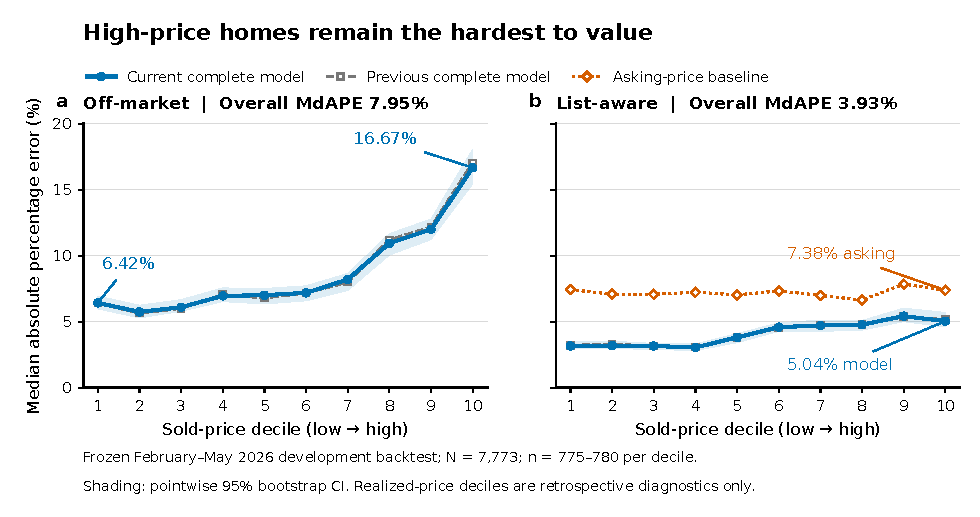
\includegraphics[width=\textwidth,height=133mm,keepaspectratio]{assets/result-price-deciles.pdf}
\par\vspace{2mm}
{\fontsize{21}{26}\selectfont\color{Teal}\bfseries Use extra review for expensive or unusual homes.}
\end{frame}

% 7 -- Close. Target: 25 seconds.
\begin{frame}[t]{Use the estimate with its limits}
\relax
\vspace{9mm}
\noindent\makebox[7cm][l]{\color{Blue}\bfseries Before listing}Off-market supports initial valuation.\par
\vspace{7mm}
\noindent\makebox[7cm][l]{\color{Teal}\bfseries After listing}List-aware adjusts the asking-price anchor.\par
\vspace{7mm}
\noindent\makebox[7cm][l]{\color{Orange}\bfseries Extra review}Expensive, unusual or weakly supported homes.\par
\vspace{13mm}
\textbf{Next:} unused-period testing and past-only uncertainty intervals.
\vfill
{\fontsize{25}{31}\selectfont\color{Teal}\bfseries Official monthly MdAPE: 7.62\% / 3.93\%}

{\smalltext\color{Muted}Hidden-test accuracy unknown. Fitted explanations describe model behaviour, not causal effects.}
\end{frame}

\ifdefined\WithAppendix
\pdfstringdefDisableCommands{\def\translate#1{#1}}
\appendix

% A -- Fitting details, outside the timed presentation.
\begin{frame}[t]{Backup A: frozen models and fitting}
\relax
\begin{columns}[T,onlytextwidth]
\begin{column}{0.52\textwidth}
\textbf{Off-market routing}

{\fontsize{16}{20}\selectfont
\renewcommand{\arraystretch}{1.35}
\begin{tabular}{@{}p{5.2cm}p{8.5cm}@{}}
\toprule
\textbf{Prediction type} & \textbf{Model / training pool}\\
\midrule
Condo Apt / Co-Op & CatBoost / shared apartments\\
Condo Townhouse & LightGBM / own type\\
Detached & LightGBM / all freehold\\
Semi-Detached & LightGBM / Semi + Freehold TH\\
Freehold Townhouse & LightGBM / all freehold\\
\bottomrule
\end{tabular}}\par\vspace{3mm}

\smalltext Related pools add examples; separate routes allow different price relationships.
\end{column}
\begin{column}{0.43\textwidth}
\textbf{Frozen LightGBM settings}

{\fontsize{16}{20}\selectfont
\renewcommand{\arraystretch}{1.35}
\begin{tabular}{@{}lrrr@{}}
\toprule
\textbf{Route} & \textbf{Trees} & \textbf{Leaves} & Rate\\
\midrule
Detached & 830 & 11 & .08206\\
Semi-Detached & 867 & 59 & .05369\\
Freehold TH & 386 & 18 & .14491\\
Condo TH & 359 & 15 & .05579\\
List-aware & 680 & 21 & .04208\\
\bottomrule
\end{tabular}}\par\vspace{3mm}

\smalltext Global List-aware: six types, 150 inputs. One model shares information and permits type interactions.
\end{column}
\end{columns}
\vfill
{\smalltext All branches use L1 on their transformed targets. Fixed configurations; no evaluation-label early stopping. Definitions, routes and settings remain fixed for the final through-May refit.}

\sourceline{Source: v17 report, Appendix A; current model schemas. TH = townhouse; leaves = maximum leaves. Displayed rates are rounded; saved schemas retain exact values.}
\end{frame}

% B -- Full same-ID comparisons, including small non-significant changes.
\begin{frame}[t]{Backup B: complete-model comparisons}
\relax
{\smalltext Same 7,773 homes and January-end frozen information set. Gap = row MdAPE minus current model in that track.}\par
\vspace{3mm}
{\fontsize{18}{23}\selectfont
\renewcommand{\arraystretch}{1.35}
\noindent\begin{tabular*}{\textwidth}{@{}l@{\extracolsep{\fill}}rrr@{}}
\toprule
\textbf{Track / complete model} & \textbf{MdAPE} & \textbf{MAPE} & \textbf{Gap, pp}\\
\midrule
Off-market: previous enhanced & 7.999\% & 10.401\% & +0.050\\
\textcolor{Blue}{Off-market: current routed trees} & \textbf{7.950\%} & 10.379\% & 0.000\\
List-aware: asking price & 7.195\% & 8.032\% & +3.261\\
List-aware: previous ratio & 3.939\% & 5.185\% & +0.005\\
\textcolor{Teal}{List-aware: current global ratio} & \textbf{3.934\%} & 5.190\% & 0.000\\
\bottomrule
\end{tabular*}}\par
\vspace{6mm}
{\smalltext\textbf{Paired 95\% intervals for current-minus-reference MdAPE:}

Off-market vs previous: $[-0.17,+0.07]$ pp\quad\textbullet\quad List-aware vs previous: $[-0.05,+0.06]$ pp

List-aware vs asking price: $[-3.44,-3.07]$ pp. Small gains over preceding models are uncertain.}
\vfill
\sourceline{Source: v17 report, Appendix F. 2,000 paired row resamples; intervals omit temporal dependence and repeated selection bias. Overall MdAPE is computed across individual homes.}
\end{frame}

% C -- Explanation must not imply causal effects or confuse final/evaluation models.
\begin{frame}[t]{Backup C: explaining one prediction}
\relax
{\smalltext ID-selected Detached example SYN-0000026\quad\textbullet\quad Asking price: \$1,688,200}

{\smalltext January-cutoff evaluation models; case selected without examining errors.}\par
\vspace{5mm}
{\fontsize{19}{24}\selectfont
\renewcommand{\arraystretch}{1.4}
\noindent\begin{tabular*}{\textwidth}{@{}l@{\extracolsep{\fill}}rr@{}}
\toprule
\textbf{Component} & \textbf{Off-market log price} & \textbf{List-aware log ratio}\\
\midrule
Expected-value term & +14.1492 & $-0.0077$\\
Sum of feature contributions & $-0.1627$ & $-0.0791$\\
Reconstructed price & \textcolor{Blue}{\textbf{\$1,186,505}} & \textcolor{Teal}{\textbf{\$1,547,898}}\\
\bottomrule
\end{tabular*}}\par
\vspace{7mm}
\takeaway{Full-precision contributions exactly reconstruct archived predictions.}

{\smalltext Correlated inputs share credit. Asking price also multiplies List-aware output outside the trees. Explanations describe fitted behaviour, not causal effects or guaranteed accuracy.}
\vfill
\sourceline{Source: v17 report, Appendix C. Display values rounded. The explanation expected value differs from the initial boosting score. These evaluation models differ from the final refits.}
\end{frame}

% D -- Updated source and reproduction status, outside the timed talk.
\begin{frame}[t]{Backup D: sources and reproducibility}
\relax
{\fontsize{17}{22}\selectfont
\textbf{Report and evidence}

Report v17. Official monthly predictions and metrics, fixed-four-month comparisons, current model index and the unchanged November 7 price-decile figure.

\textbf{Team code and both forecasts}

\href{https://github.com/hmengfan693/SSU-Data-Dash-2026}{github.com/hmengfan693/SSU-Data-Dash-2026}

{\fontsize{15}{20}\selectfont
\texttt{python run.py validate --data-dir /path/to/data --output /new/run}\par
\texttt{python verify\_official\_validation.py --data-dir /path/to/data --output /new/run}\par}

Six monthly folds fit 42 models. Every February prediction exactly reproduces the indexed model at the same training cutoff. Final forecasts retain 3,974 Off-market and 4,064 List-aware rows.

\textbf{Competition and method sources}

\href{https://github.com/erwinzhang7/SSU-Data-Dash/blob/main/handout.md}{Official handout}\quad
\href{https://github.com/erwinzhang7/SSU-Data-Dash/blob/main/run.py}{Official monthly split and scoring}\quad
\href{https://huggingface.co/datasets/Baliyang/SSU_data_dash}{Competition dataset}\quad
\href{https://lightgbm.readthedocs.io/en/stable/Features.html}{LightGBM feature guide}
}
\vfill
\sourceline{Configuration selection overlapped December 2025. Both protocols are cumulative development validation. Hidden-test error and competition points remain unknown. Repository updates do not submit the organizer's form.}
\end{frame}
\fi
\end{document}
